% English combined report. Build: tectonic -X compile report_en.tex  (in rapor\ ; fonts in ../fontlar ; names in isimler.tex, not tracked)
\documentclass[10.5pt,a4paper]{article}
% Ortak onbilgi: uc "Study of Simulation Tools" raporu icin. Derleme: tectonic -X compile <dosya>.tex (rapor\ klasorunde)
\usepackage{fontspec}
\setmainfont{georgia}[Path=../fontlar/,Extension=.ttf,BoldFont=georgiab,ItalicFont=georgiai,BoldItalicFont=georgiaz]
\setsansfont{arial}[Path=../fontlar/,Extension=.ttf,BoldFont=arialbd,ItalicFont=ariali,BoldItalicFont=arialbi]
\setmonofont{consola}[Path=../fontlar/,Extension=.ttf,BoldFont=consolab,ItalicFont=consolai,BoldItalicFont=consolaz,Scale=0.86]
\usepackage[a4paper,left=2.2cm,right=2.2cm,top=1.9cm,bottom=1.8cm]{geometry}
\usepackage{xcolor,graphicx,titlesec,enumitem,amsmath,booktabs,xltabular,listings,fancyhdr,caption}
\emergencystretch=3em
\definecolor{ink}{HTML}{1F2937}\definecolor{acc}{HTML}{1D4ED8}\definecolor{muted}{HTML}{6B7280}\definecolor{codebg}{HTML}{F3F4F6}
\color{ink}
\titleformat{\section}{\sffamily\bfseries\large\color{acc}}{}{0pt}{}
\titlespacing*{\section}{0pt}{9pt}{3pt}
\titleformat{\subsection}{\sffamily\bfseries\normalsize}{}{0pt}{}
\titlespacing*{\subsection}{0pt}{6pt}{2pt}
\setlength{\parindent}{0pt}\setlength{\parskip}{4pt plus 1pt}
\setlist{itemsep=1pt,topsep=2pt,parsep=0pt}
\pagestyle{fancy}\fancyhf{}\renewcommand{\headrulewidth}{0.3pt}
\fancyhead[L]{\sffamily\footnotesize\color{muted} EHB415 \textbullet\ Study of Simulation Tools}
\fancyfoot[C]{\sffamily\footnotesize\color{muted}\thepage}
\captionsetup{font={sf,footnotesize},labelfont=bf,labelsep=period,skip=2pt}
\lstset{basicstyle=\ttfamily\footnotesize,backgroundcolor=\color{codebg},frame=single,rulecolor=\color{codebg!70!black},
  breaklines=true,columns=fullflexible,keepspaces=true,showstringspaces=false,aboveskip=4pt,belowskip=6pt,
  literate={ğ}{g}1 {ş}{s}1 {ı}{i}1 {ü}{u}1 {ö}{o}1 {ç}{c}1}
\newcommand{\baslik}[2]{%
  {\sffamily\color{muted}\small EHB415 Dönem Projesi \textbullet\ 2026--2027 Güz\par}
  {\sffamily\bfseries\Large Study of Simulation Tools: #1\par}
  {\sffamily\small #2\par}
  \vspace{-2pt}{\color{acc!40}\rule{\textwidth}{0.8pt}}\par}
\IfFileExists{isimler.tex}{\input{isimler}}{\newcommand{\taha}{[Ad Soyad -- No]}\newcommand{\aziz}{[Ad Soyad -- No]}\newcommand{\fatih}{[Ad Soyad -- No]}\newcommand{\nihat}{[Ad Soyad -- No]}}

\usepackage{float}
\titleformat{\section}{\sffamily\bfseries\large\color{acc}}{\thesection.}{0.5em}{}
\titleformat{\subsection}{\sffamily\bfseries\normalsize}{\thesubsection}{0.5em}{}
\titleformat{\subsubsection}{\sffamily\bfseries\small\color{ink}}{}{0pt}{}
\titlespacing*{\subsubsection}{0pt}{5pt}{2pt}
% code blocks never split across pages
\newenvironment{codebox}{\par\noindent\begin{minipage}{\textwidth}}{\end{minipage}\par}
\begin{document}

% ------------------------------------------------------------------ COVER
\thispagestyle{empty}
\begin{center}
\vspace*{3.2cm}
{\bfseries\LARGE EHB415E\par}
\vspace{1.2cm}
{\bfseries\LARGE Term Project\par}
\vspace{2.2cm}
{\large 2026--2027 Fall Semester -- Project Report\par}
\vspace{0.5cm}
{\large Study of Simulation Tools\par}
\vspace{1.6cm}
{\bfseries\Large Integrating Sensing Capabilities into 5G Networks:\\ An ISAC-Oriented Study\par}
\vspace{2.6cm}
{\large \taha\par\vspace{4pt} \aziz\par\vspace{4pt} \fatih\par\vspace{4pt} \nihat\par}
\end{center}
\clearpage

% ------------------------------------------------------------------ 1
\section{Project Context and Scope of This Report}
Integrated sensing and communication (ISAC) is an emerging approach in which wireless infrastructure both carries data and senses its surroundings. Adding sensing to 5G-Advanced and 6G networks raises questions about resource allocation, processing load and the resulting impact on communication performance. Our project investigates how ISAC functions can be incorporated into an open-source 5G network architecture (OCUDU) and evaluates their effects with simulation tools. The objectives are: (i) to review 3GPP ISAC studies, (ii) to investigate how selected functions could be implemented within or alongside OCUDU, (iii) to build a simulation-based evaluation framework, and (iv) to evaluate the trade-off between sensing and communication performance.

This report shows that the three tools we will use are \textbf{installed correctly and working}: \textbf{ns-3 with 5G-LENA}, \textbf{OCUDU} and \textbf{Sionna}. The tools look at one question from three sides: \emph{if we give the sensing function a share of the radio resources, what does sensing gain and what does communication lose?} The common axis is the share of resources given to sensing ($\alpha$).

\begin{center}\sffamily\small
\begin{tabular}{@{}p{2.6cm}p{3.2cm}p{3.5cm}p{4.0cm}@{}}
\toprule
\textbf{Tool} & \textbf{Role in project} & \textbf{Version / environment} & \textbf{Verification} \\
\midrule
ns-3 + 5G-LENA & Cost on communication (network level) & ns-3.48, nr v5.1; WSL2 Ubuntu 24.04 & \texttt{cttc-nr-demo} ran; our own program matched a hand calculation \\
OCUDU & Cost on communication (real gNB code) & 26.10.0; WSL2 Ubuntu 24.04, Clang 18 & \texttt{testmode}: DL $\approx$59 Mbps, UL 77.3 Mbps, 1000 blocks/s \\
Sionna / Sionna RT & Sensing gain (channel and radar) & 1.2.2; Ubuntu 22.04 and Windows 11 & Radar test within resolution; ray tracing found 12 paths \\
\bottomrule
\end{tabular}
\end{center}

% ------------------------------------------------------------------ 2 ns-3
\section{ns-3 and 5G-LENA}
\subsection{Role in the project and why we chose it}
In our project ns-3 measures the cost on communication \textbf{in a multi-user network}: how throughput and delay change as the number of users grows. ns-3 is an open-source network simulator. \textbf{5G-LENA} (the \texttt{nr} module) developed by CTTC is added to ns-3 to simulate 5G NR. We chose it because it includes the MAC-layer schedulers of 5G NR, ships ready-made 5G examples, and can measure throughput and delay per flow. 5G-LENA recommends a specific ns-3 version for each release; we use the pair \textbf{ns-3.48 + 5G-LENA v5.1}.

\subsection{Installation}
\begin{center}\sffamily\small
\begin{tabular}{@{}ll@{}}
\toprule
Environment & WSL2 on Windows 11, Ubuntu 24.04.5 LTS \\
Compiler and tools & g++ 13.3.0, CMake 3.28.3, Ninja \\
Simulator & ns-3.48 (\texttt{\textasciitilde/ehb415/ns-3-dev}) \\
5G module & 5G-LENA v5.1 (\texttt{contrib/nr}) \\
Build profile & optimized (\texttt{-d optimized}), 1876 targets \\
Time and disk & about 18 minutes (\texttt{-j6}), about 0.5 GB \\
\bottomrule
\end{tabular}
\end{center}
\begin{codebox}Installation commands (in the Ubuntu terminal):\par
\begin{lstlisting}
sudo apt-get update
sudo apt-get install -y build-essential g++ python3 python3-venv python3-pip cmake \
    ninja-build git ccache pkg-config libc6-dev sqlite3 libsqlite3-dev libeigen3-dev
mkdir -p ~/ehb415 && cd ~/ehb415
git clone --depth 1 --branch ns-3.48 https://gitlab.com/nsnam/ns-3-dev.git
git clone --depth 1 --branch v5.1 https://gitlab.com/cttc-lena/nr.git ns-3-dev/contrib/nr
cd ns-3-dev
./ns3 configure --enable-examples -d optimized -G Ninja
./ns3 build -j6
\end{lstlisting}
\end{codebox}
The 5G-LENA folder must be named \texttt{nr} and placed under \texttt{contrib/}.

\subsection{Problems encountered and solutions}
\begingroup\sffamily\small
\begin{xltabular}{\textwidth}{@{}p{4.3cm}X@{}}
\toprule
\textbf{Problem} & \textbf{Cause and solution} \\
\midrule
\texttt{WSL2 is unable to start since virtualization is not enabled} & A real restart had not been done after installing WSL. With Fast Startup enabled, shutting down and powering on is not enough. Solved with \textbf{Start $\rightarrow$ Power $\rightarrow$ Restart}. \\
\texttt{Killed} during the build & Not enough memory. \texttt{memory=10GB} was set in \texttt{.wslconfig} and the job count was lowered (\texttt{-j4} or \texttt{-j2}) when needed. \\
Complex \texttt{wsl -- bash -c '...'} commands break when run from PowerShell & Quotes and characters such as \texttt{\$} and \texttt{|} get mixed up between PowerShell and bash. The commands were written to a \texttt{.sh} file and run with \texttt{wsl -- bash file.sh}. \\
No \texttt{NS\_LOG} messages in the simulation output & In the ``optimized'' profile the log output is compiled out. Results are read from the flow monitor (FlowMonitor) and \texttt{trace} callbacks instead. If logs are needed, reconfigure with \texttt{-d debug}. \\
Building with another ns-3 version & 5G-LENA v5.1 is designed for ns-3.48; versions such as ns-3.49 should not be used. \\
\bottomrule
\end{xltabular}
\endgroup

\subsection{Example runs}
\subsubsection*{The ready-made 5G-LENA example: \texttt{cttc-nr-demo}}
To check the installation, we ran the 5G-LENA example with 2 users (UEs) for a 1-second simulation.
\begin{figure}[H]
\centering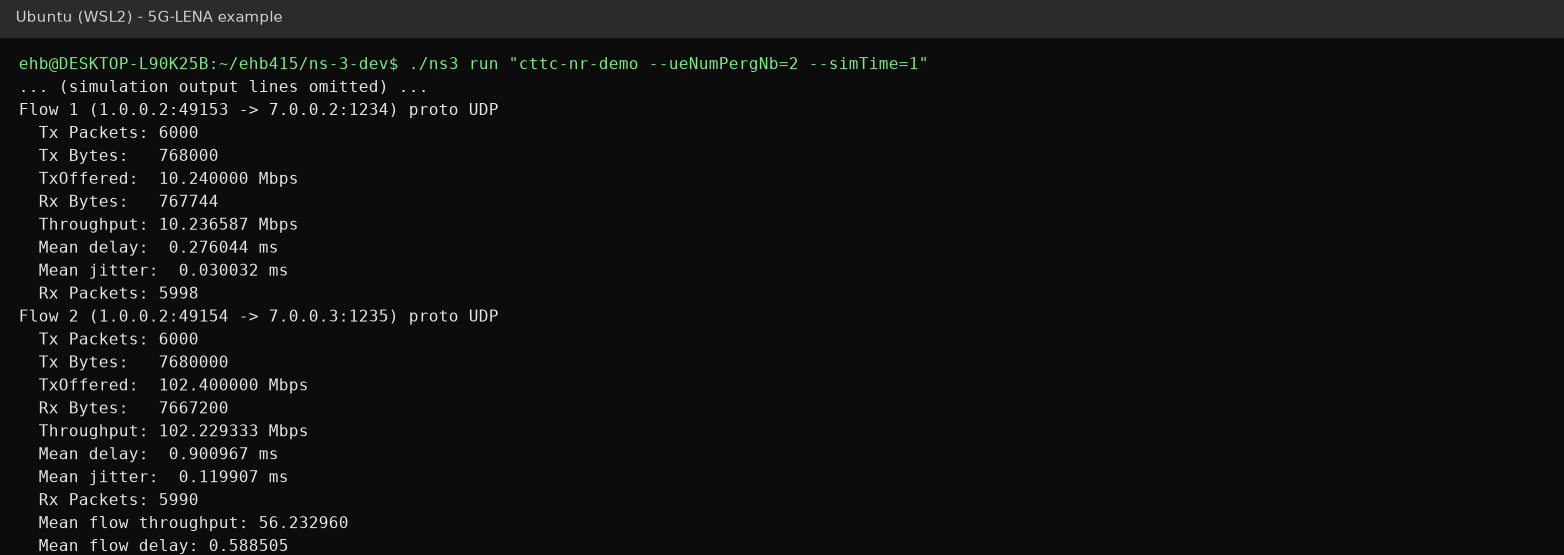
\includegraphics[width=0.88\textwidth]{img/ns3_rapor_demo.png}
\caption{Flow results of \texttt{cttc-nr-demo} (WSL2 Ubuntu terminal).}
\end{figure}
\begin{center}\sffamily\small
\begin{tabular}{@{}lrrrr@{}}
\toprule
 & Sent & Received & Delay & Packet loss \\
\midrule
Flow 1 & 10.24 Mbps & 10.24 Mbps & 0.28 ms & 0.03\% \\
Flow 2 & 102.40 Mbps & 102.23 Mbps & 0.90 ms & 0.17\% \\
Mean (\texttt{Mean flow}) & & 56.23 Mbps & 0.59 ms & \\
\bottomrule
\end{tabular}
\end{center}
The received data is very close to the sent data and the delay is below 1\,ms. This is expected because the load is below the capacity.

\subsubsection*{A simple application we wrote ourselves}
To understand how ns-3 works, we wrote a program with two computers connected by a cable (\texttt{scratch/benim\_ilk.cc}). The cable runs at 5\,Mbps with 500\,ms delay; the client sends a single 1024-byte packet at t\,=\,2\,s and the server replies.
\begin{figure}[H]
\centering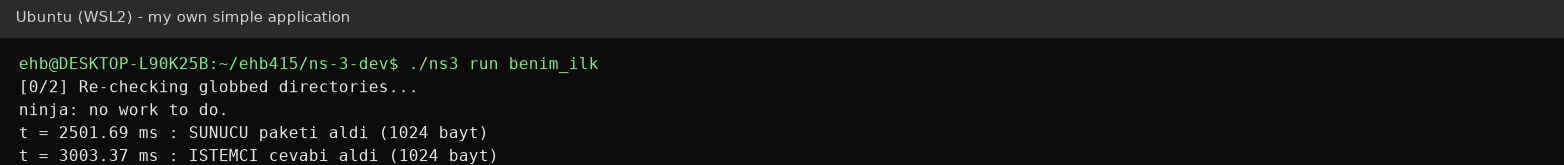
\includegraphics[width=0.88\textwidth]{img/ns3_rapor_ilk.png}
\caption{Output of \texttt{./ns3 run benim\_ilk} (SUNUCU = server, ISTEMCI = client, paketi aldi = received the packet).}
\end{figure}
By hand: 1054 bytes including headers, $1054\times 8/5\,\text{Mbps}=1.69$\,ms transmission time plus 500\,ms cable delay $=501.69$\,ms. The server received the packet at $2000+501.69=2501.69$\,ms and, since the reply travels the same path, the client received it at $3003.37$\,ms. The simulation output matched the hand calculation exactly.

\subsection{Assessment and next steps}
ns-3.48 and 5G-LENA v5.1 were installed and compiled, and both the ready-made 5G example and our own program gave correct results. Limitation: 5G-LENA has no ready-made sensing model, so ns-3 will only measure the cost on the communication side; the way to represent the sensing load in the simulation has not been chosen yet. Next steps:
\begin{itemize}
\item Vary the number of users (1, 2, 5, 10, 20) and measure total throughput and delay.
\item Study the schedulers in 5G-LENA (\texttt{nr-mac-scheduler-*}); the default is \texttt{NrMacSchedulerTdmaRR}.
\item Run an experiment that imitates the sensing load by narrowing the bandwidth and compare it with the alternative of adding sensing as a separate traffic flow.
\end{itemize}

% ------------------------------------------------------------------ 3 OCUDU
\section{OCUDU}
\subsection{Role in the project and why we chose it}
OCUDU is an open-source \textbf{real 5G base station (gNB) software}, the successor of the srsRAN Project, developed under the Linux Foundation. It is real protocol code, not a model like ns-3. In our project it will be used to measure the cost of the resources given to sensing (PRS) on communication in a real scheduler, which adds credibility to the ns-3 results. To run without a real radio (USRP) we used ZeroMQ (virtual RF) and \texttt{testmode}.

\subsection{Installation}
\begin{center}\sffamily\small
\begin{tabular}{@{}ll@{}}
\toprule
Environment & WSL2 on Windows 11, Ubuntu 24.04.5 LTS \\
Compiler and tools & Clang 18.1.3, CMake 3.28.3, ccache \\
Software version & OCUDU \texttt{release\_26\_10}, 26.10.0 (commit e0db566) \\
Options & \texttt{ENABLE\_ZEROMQ=ON}, \texttt{ENABLE\_EXPORT=ON}; only the \texttt{gnb} target \\
Time and disk & about 23 minutes (\texttt{-j4}), about 0.6 GB \\
\bottomrule
\end{tabular}
\end{center}
The official installation page recommends gcc 15.2 or newer, or Clang 14 or newer. Ubuntu 24.04 ships gcc 13.3, so we used \textbf{Clang 18}.\begin{codebox}Commands:\par
\begin{lstlisting}
sudo apt-get update
sudo apt-get install -y cmake make gcc g++ clang pkg-config \
    libmbedtls-dev libsctp-dev libyaml-cpp-dev libgtest-dev \
    libfftw3-dev libeigen3-dev libzmq3-dev ccache
mkdir -p ~/ehb415 && cd ~/ehb415
git clone --depth 1 --branch release_26_10 https://gitlab.com/ocudu/ocudu.git
cd ocudu && mkdir -p build && cd build
CC=clang CXX=clang++ cmake ../ -DENABLE_EXPORT=ON -DENABLE_ZEROMQ=ON \
    -DCMAKE_C_COMPILER_LAUNCHER=ccache -DCMAKE_CXX_COMPILER_LAUNCHER=ccache
make -j4 gnb
\end{lstlisting}
\end{codebox}
The CMake output should contain the lines \texttt{The CXX compiler identification is Clang 18.1.3} and \texttt{Found libZEROMQ}.

\subsection{Problems encountered and solutions}
\begingroup\sffamily\small
\begin{xltabular}{\textwidth}{@{}p{4.3cm}X@{}}
\toprule
\textbf{Problem} & \textbf{Cause and solution} \\
\midrule
\texttt{Found libZEROMQ} missing in the CMake output & ZeroMQ is detected only at configure time. \texttt{libzmq3-dev} was installed, the \texttt{build} folder was deleted and \texttt{cmake} was run again. \\
The word ``error'' in the build output & It appears in file names (\texttt{..\_error\_handler\_impl.cpp}). A real error starts with \texttt{error:} and gives a file:line location. \\
\texttt{256QAM MCS table cannot be used for PDSCH with fallback DCI format} & In the first testmode attempt the setting \texttt{pdsch/pusch mcs\_table: qam64} was missing. After adding it to the configuration file the cell came up. \\
\texttt{Scheduling priority of thread ... not changed. Not enough privileges} & Real-time priority needs \texttt{sudo}. It is harmless under WSL and did not prevent the cell from starting. \\
\texttt{Real-time failure in RU: received late DL request} in the log & Expected, because the WSL2 kernel is not real-time. \\
The metrics table is not shown & The table appears only in an interactive terminal (TTY). While the program is running, type \texttt{t} and press Enter. \\
\bottomrule
\end{xltabular}
\endgroup

\subsection{Example run}
To verify the installation we ran the gNB without a radio or a core network (\texttt{ru\_dummy}, \texttt{no\_core}, one virtual user; configuration file: \texttt{ocudu\_testmode.yml}). After the program started we typed \texttt{t} and pressed Enter to open the live metrics table.
\begin{codebox}
\begin{lstlisting}
cd ~/ehb415/ocudu/build/apps/gnb
./gnb --version
./gnb -c ~/ehb415/ocudu_testmode.yml
\end{lstlisting}
\end{codebox}
\begin{figure}[H]
\centering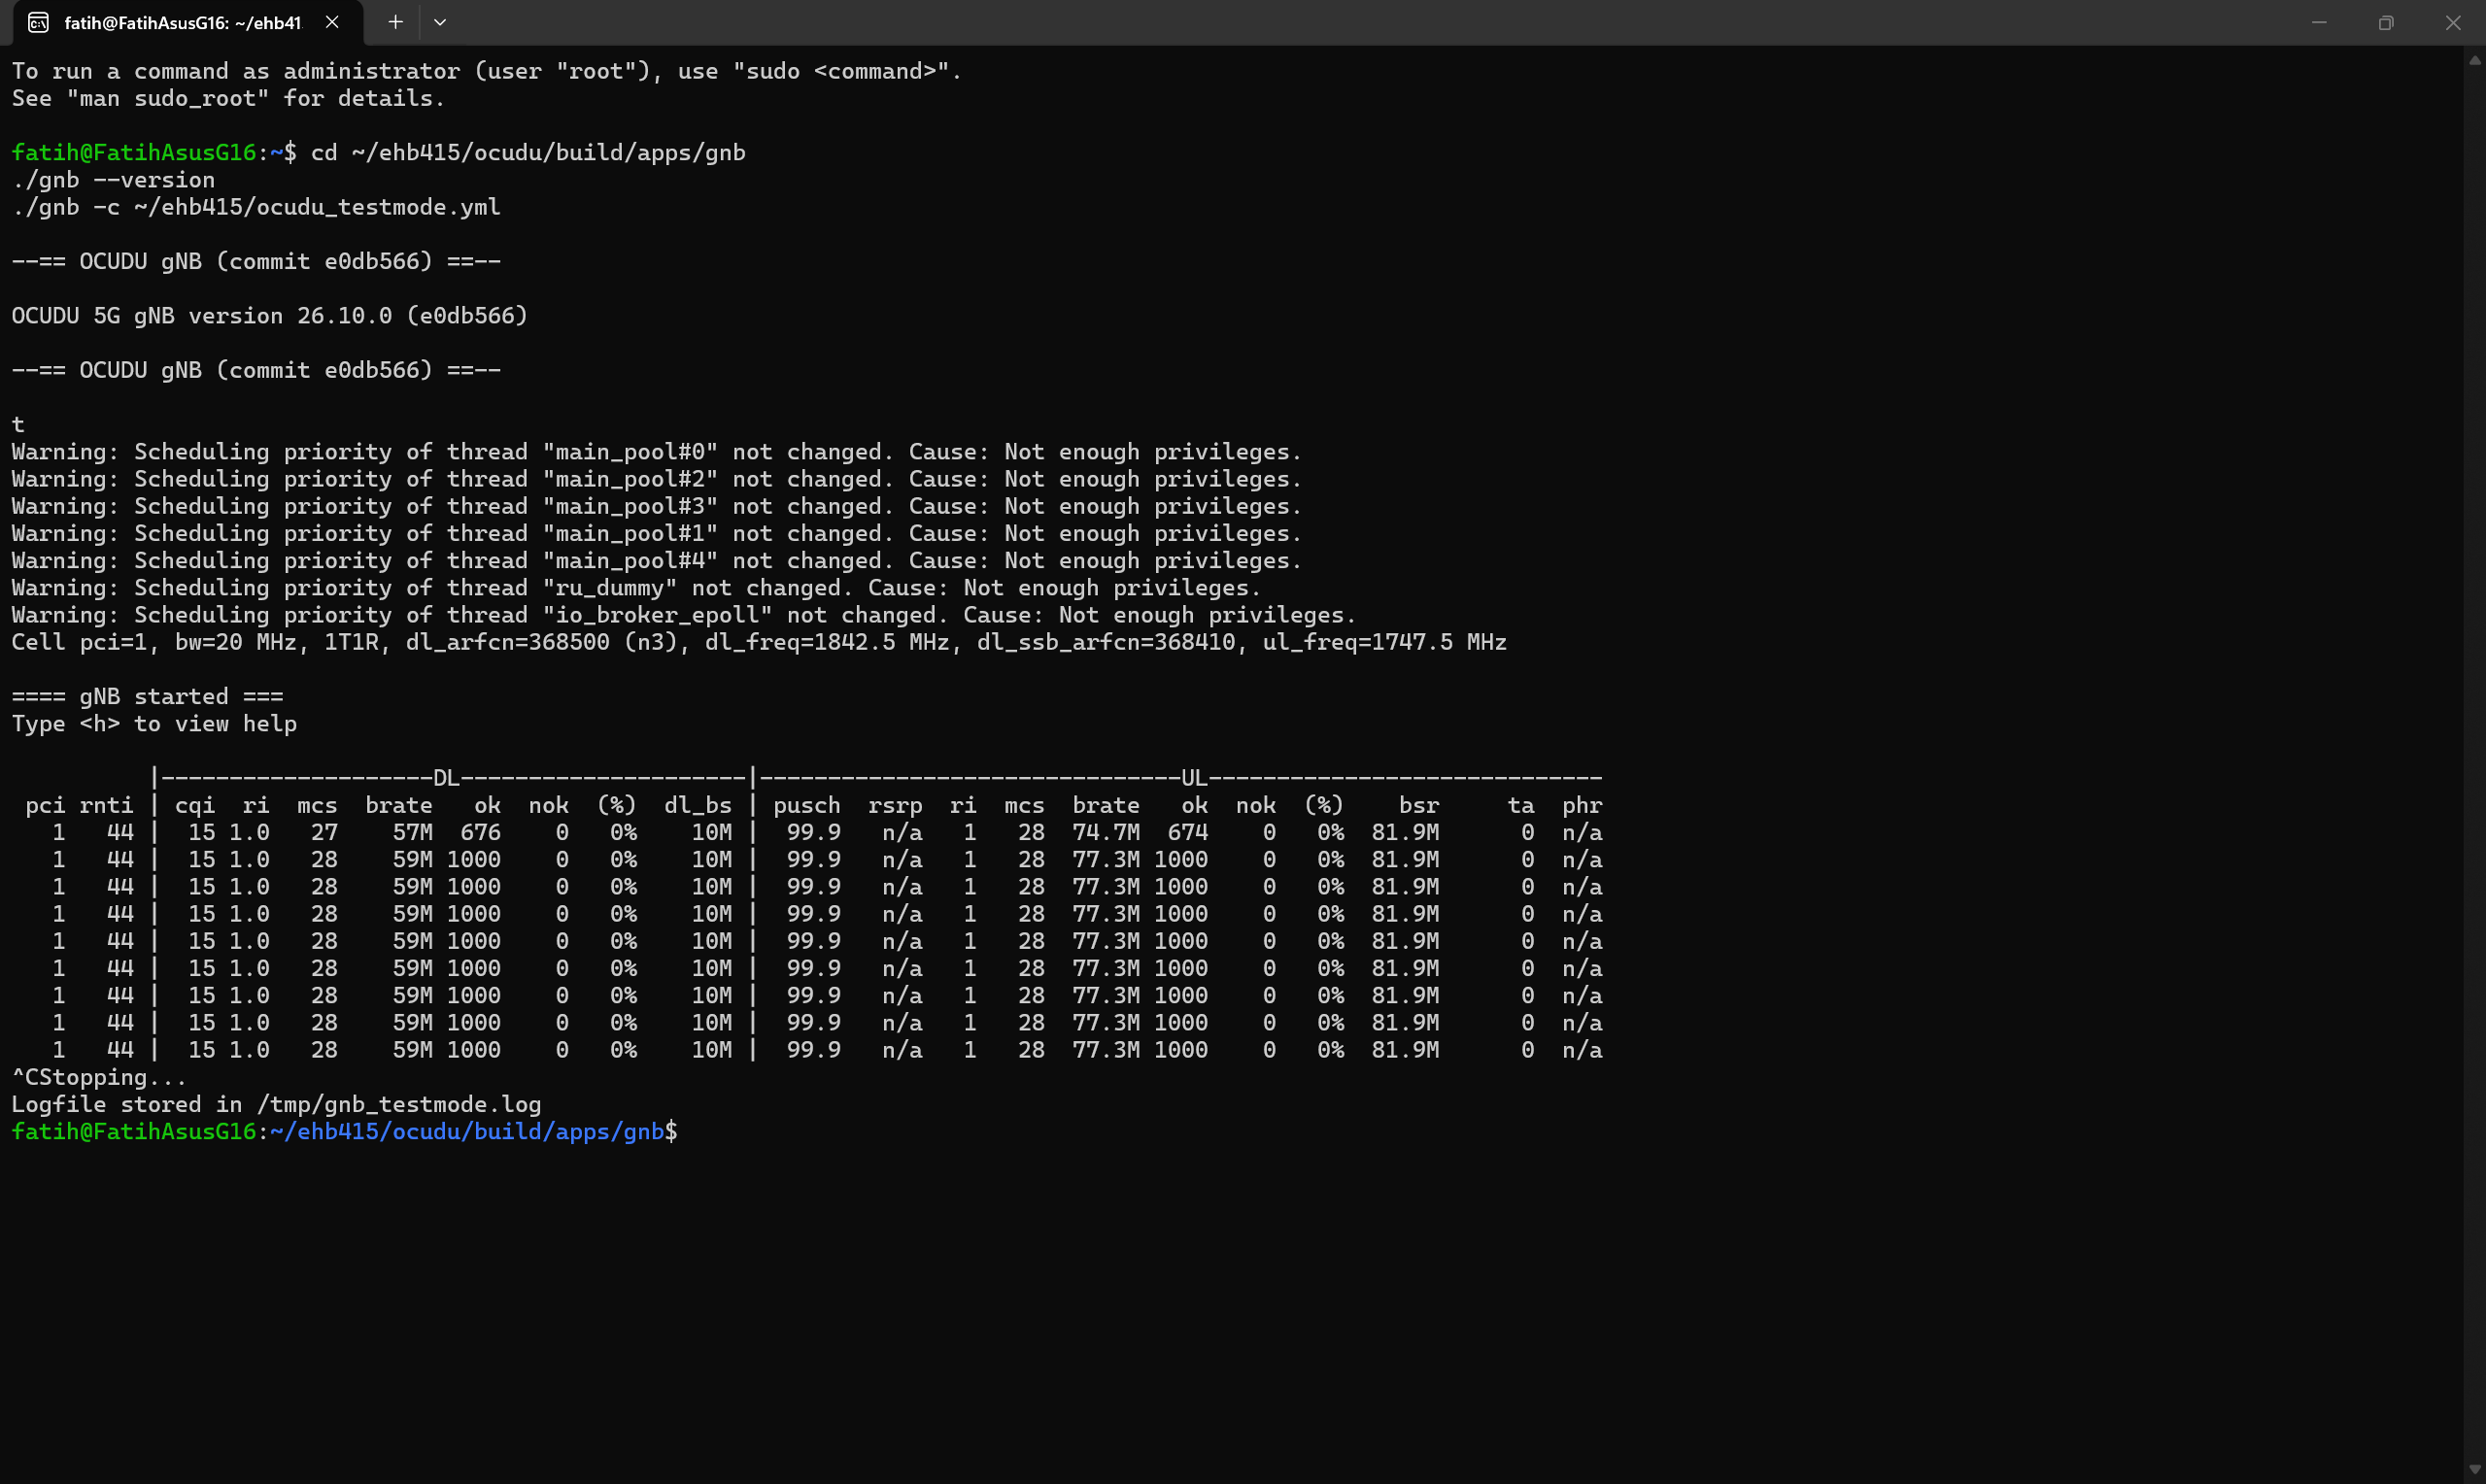
\includegraphics[width=0.86\textwidth]{img/ocudu_terminal.png}
\caption{\texttt{gnb --version}, the cell coming up and the live metrics table (WSL2 Ubuntu).}
\end{figure}
The output shows version 26.10.0 (e0db566) and a cell in band n3 with 20\,MHz and 1T1R. In the stable rows of the table the \textbf{DL rate is about 59 Mbps, the UL rate is 77.3 Mbps} and the number of successful blocks is \textbf{1000 blocks/s} in both directions. After Ctrl+C the program shut down cleanly with a \texttt{Stopping} message. These outputs show that OCUDU runs in the radio-less test environment and produces measurements.

\subsection{Assessment and next steps}
OCUDU 26.10.0 was built and ran in testmode. Limitations: (i) the end-to-end test with srsUE and Open5GS was \textbf{not performed}; it was taken from the official documentation and was not run in this installation. (ii) WSL2 is not real-time, so a real radio (USRP) connection is not supported; the project does not need it. Next steps:
\begin{itemize}
\item Change the PRS (positioning reference signal) period and measure the drop in DL rate (59.0 Mbps without PRS).
\item Repeat the same experiment with several virtual users.
\item Open question: why does a 4-symbol PRS cause the same loss as a 12-symbol PRS? We will examine which symbol range the scheduler code (\texttt{intra\_slice\_scheduler.cpp}) checks for PDSCH.
\end{itemize}

% ------------------------------------------------------------------ 4 Sionna
\section{Sionna and Sionna RT}
\subsection{Role in the project and why we chose it}
Sionna is NVIDIA's open-source link-level simulation library; \textbf{Sionna RT} computes the channel in a real city scene using ray tracing. In the project Sionna measures the \textbf{sensing gain}: as the resource share $\alpha$ given to sensing grows, from what distance, with what probability and how accurately can a UAV be found? Sionna RT provides a realistic scenario (the Munich scene, 4.9\,GHz) in which buildings block the line of sight. Because ns-3 and OCUDU measure only the cost, no trade-off can be derived without measuring the gain.

\subsection{Installation}
The installation was done in two environments and gave the same package versions in both.
\begin{center}\sffamily\small
\begin{tabular}{@{}lll@{}}
\toprule
 & \textbf{Environment A: Ubuntu} & \textbf{Environment B: Windows} \\
\midrule
Operating system & Ubuntu 22.04.5 LTS & Windows 11 \\
Python & system Python 3.10.12 & 3.11.9 (virtual environment) \\
LLVM (for Sionna RT) & \texttt{libllvm14} (apt) & LLVM 23.1.3 (\texttt{winget}) \\
Sionna / sionna-rt & 1.2.2 / 1.2.2 & 1.2.2 / 1.2.2 \\
TensorFlow, Mitsuba, Dr.Jit & 2.21.0, 3.8.0, 1.3.1 & 2.21.0, 3.8.0, 1.3.1 \\
Time and disk & $\approx$5 min (fast network), 2.8 GB & 15--30 min, 2.1 GB \\
\bottomrule
\end{tabular}
\end{center}
\begin{codebox}\textbf{Environment A (Ubuntu) commands:}\par
\begin{lstlisting}
sudo apt update
sudo apt install -y python3-venv libllvm14 libatomic1
mkdir -p ~/venvs && python3 -m venv ~/venvs/ehb415
~/venvs/ehb415/bin/python -m pip install --upgrade pip
~/venvs/ehb415/bin/python -m pip install --retries 10 --timeout 60 "sionna==1.2.2" jupyterlab matplotlib scipy
\end{lstlisting}
\end{codebox}
\begin{codebox}\textbf{Environment B (Windows) commands} (PowerShell). Installing LLVM requires an \emph{administrator} PowerShell:\par
\begin{lstlisting}
python -m venv C:\Users\$env:USERNAME\venvs\ehb415
C:\Users\$env:USERNAME\venvs\ehb415\Scripts\python.exe -m pip install --retries 10 --timeout 60 "sionna==1.2.2" jupyterlab matplotlib scipy
.\kur-llvm.ps1      # administrator PowerShell: installs LLVM and sets DRJIT_LIBLLVM_PATH
\end{lstlisting}
\end{codebox}
Pinning \texttt{sionna==1.2.2} matters: with Python 3.11 an unpinned \texttt{pip install sionna} picks Sionna 2.2.0, and our scripts are written for 1.2.2.

\subsection{Problems encountered and solutions}
\begingroup\sffamily\small
\begin{xltabular}{\textwidth}{@{}p{4.4cm}X@{}}
\toprule
\textbf{Problem} & \textbf{Cause and solution} \\
\midrule
\texttt{ensurepip is not available} (Ubuntu) & The \texttt{python3-venv} package is missing. \texttt{sudo apt install -y python3-venv}. \\
\texttt{Could not import the Dr.Jit binary extension ... incompatible with the current interpreter} (Ubuntu) & The message is misleading: the real cause is the missing \texttt{libatomic.so.1}, not the Python version. \texttt{sudo apt install -y libatomic1}. \\
\texttt{LLVM shared library ("libLLVM.so") could not be found} (Ubuntu) & \texttt{sudo apt install -y libllvm14}. \\
\texttt{LLVM-C.dll could not be found} (Windows) & LLVM is not installed or \texttt{DRJIT\_LIBLLVM\_PATH} is not set. Run \texttt{kur-llvm.ps1} (administrator) and open a \textbf{new PowerShell} (environment variables do not reach already-open windows). \\
\texttt{free(): invalid pointer} or \texttt{Segmentation fault} at exit (Ubuntu) & TensorFlow was imported before \texttt{sionna.rt}. \texttt{import sionna.rt} must always be the \textbf{first} import. Not a problem on Windows. \\
Unexpected Sionna 2.2.0 installed with Python 3.11 & The version was not pinned. Write \texttt{"sionna==1.2.2"}. \\
\texttt{TypeError: PathSolver ... 'samples\_per\_tx'} & In Sionna 1.2.2 the parameter is named \texttt{samples\_per\_src}; older example code uses a different name. \\
\texttt{TensorFlow GPU support is not available on native Windows} & Expected and harmless warning; Sionna runs on the CPU. \\
\bottomrule
\end{xltabular}
\endgroup

\subsection{Example runs}
\subsubsection*{Installation check (Environment B, Windows)}
First we listed the package versions, then ran the two verification scripts. \texttt{sionna\_dogrulama.py} runs a single-target OFDM radar test in plain NumPy and creates Sionna's \texttt{ResourceGrid} object; \texttt{sionna\_rt\_dogrulama.py} loads the Munich scene and computes ray paths.
\begin{figure}[H]
\centering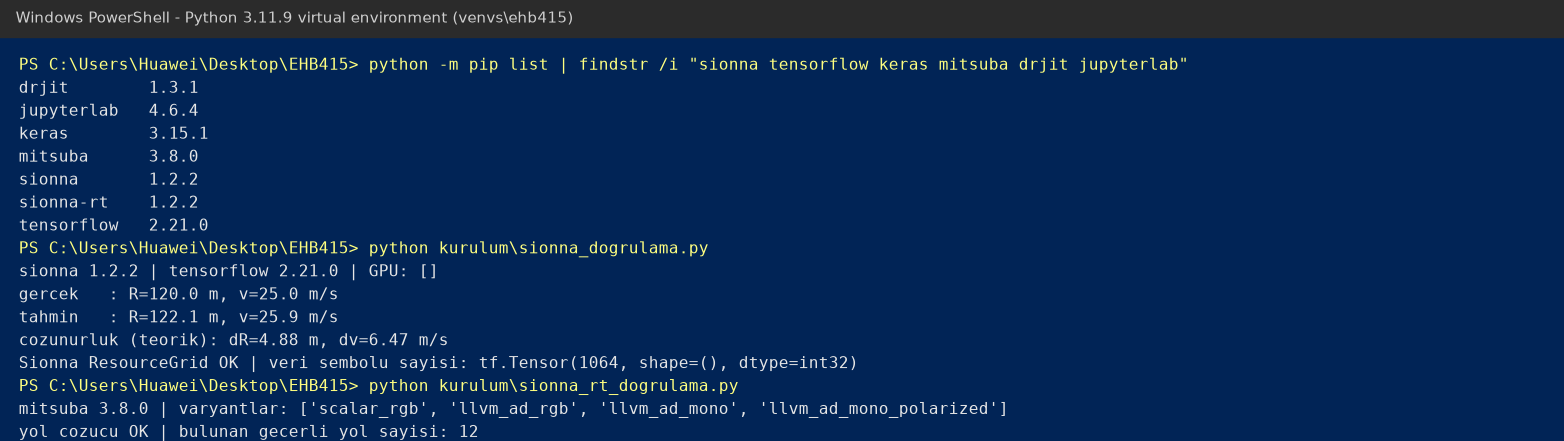
\includegraphics[width=0.88\textwidth]{img/sionna_windows_terminal.png}
\caption{Package versions and the output of the two verification scripts (Windows PowerShell). The script prints Turkish labels: gercek = true, tahmin = estimate, cozunurluk = resolution, yol cozucu = path solver.}
\end{figure}
In the radar test the true target was at 120.0\,m and 25.0\,m/s and the estimate was 122.1\,m and 25.9\,m/s; the errors are within the theoretical resolution cell (4.88\,m and 6.47\,m/s), so the result is correct. Sionna RT found 12 valid ray paths.

\subsubsection*{Project scripts (Environment A, Ubuntu)}
On Ubuntu we ran two project scripts: \texttt{radar\_takip.py} detects a UAV at different ranges with a simple radar model in which a share $\alpha$ of the symbols is given to sensing; \texttt{rt\_sehir.py} computes the radio map and ray paths in the city scene with Sionna RT.
\begin{figure}[H]
\centering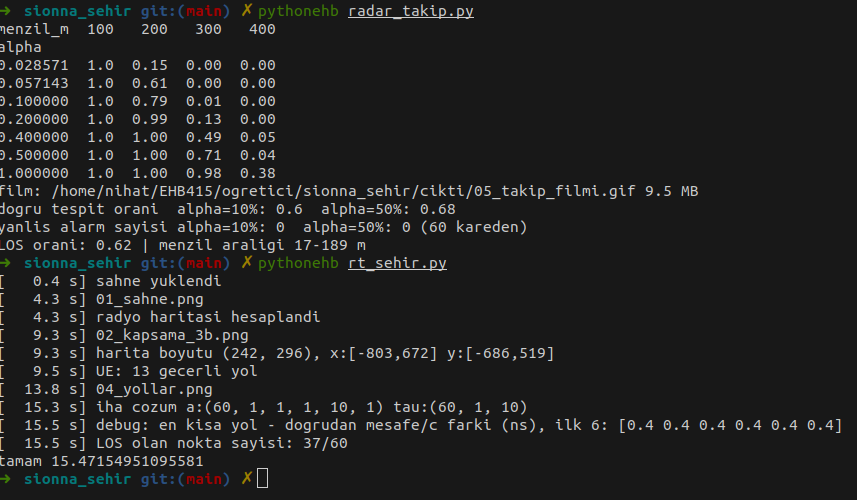
\includegraphics[width=0.7\textwidth]{img/sionna_ubuntu_terminal.png}
\caption{Detection probability table of \texttt{radar\_takip.py} (rows: $\alpha$, columns: UAV range in m) and output of \texttt{rt\_sehir.py} (Ubuntu). ``dogru tespit orani'' = correct detection rate, ``yanlis alarm sayisi'' = number of false alarms, ``LOS orani'' = line-of-sight ratio, ``menzil araligi'' = range interval.}
\end{figure}
\begin{itemize}
\item \textbf{Detection probability:} at 100\,m the UAV is found for every $\alpha$. At 200\,m the probability is 0.15 for $\alpha=2.9\%$ and 0.99 for $\alpha=20\%$. At 300\,m it reaches 0.98 only at $\alpha=100\%$; at 400\,m it is at most 0.38.
\item \textbf{Tracking scenario (60 frames):} the correct detection rate is 0.60 for $\alpha=10\%$ and 0.68 for $\alpha=50\%$; there were no false alarms.
\item \textbf{Line of sight:} in 37 of the 60 points (62\%) there is a direct line of sight between the UAV and the transmitter. That the detection rates are close to this ratio suggests that detection comes largely from frames with a direct line of sight.
\item \textbf{Sionna RT run time:} the scene loaded in 0.4\,s and all steps finished in about 15.5\,s.
\end{itemize}
\begin{figure}[H]
\centering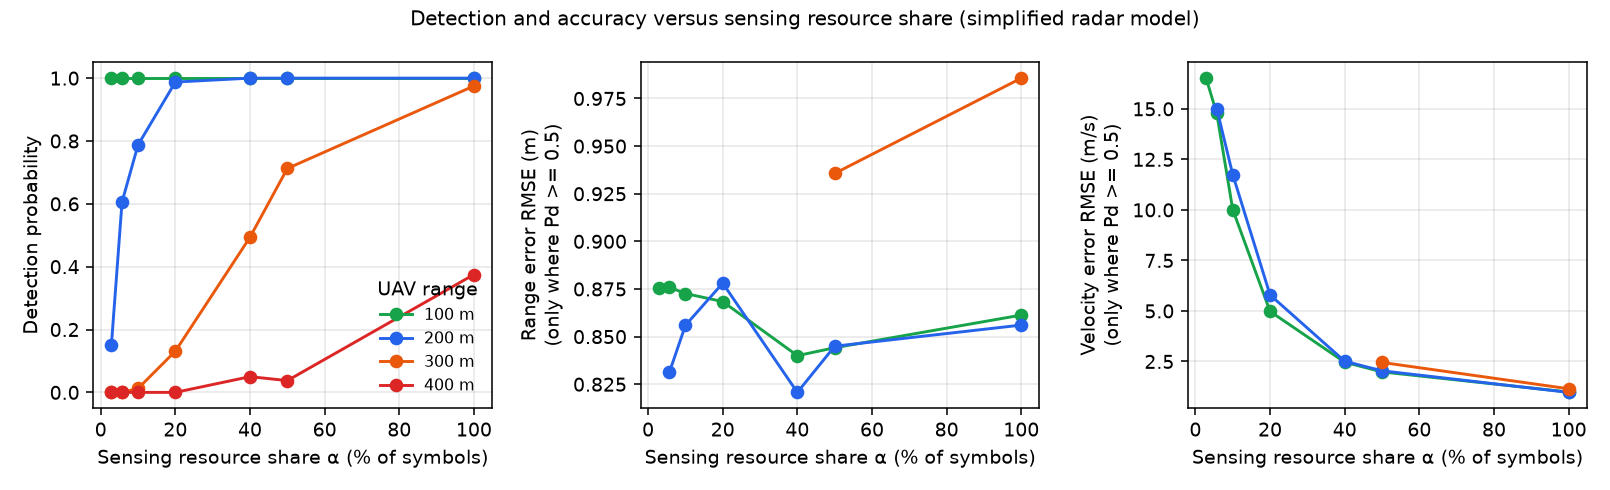
\includegraphics[width=0.95\textwidth]{img/sionna_grafik.png}
\caption{Detection probability, range error and velocity error as the sensing share $\alpha$ grows.}
\end{figure}
In the chart the range error is almost independent of $\alpha$ ($\approx$0.8--1.0\,m), while the velocity error falls from 15--16\,m/s to about 1\,m/s as $\alpha$ increases. Range resolution depends on bandwidth, not on the number of symbols, so range accuracy hardly changes; giving more symbols to sensing mainly improves velocity (Doppler) estimation.
\begin{figure}[H]
\centering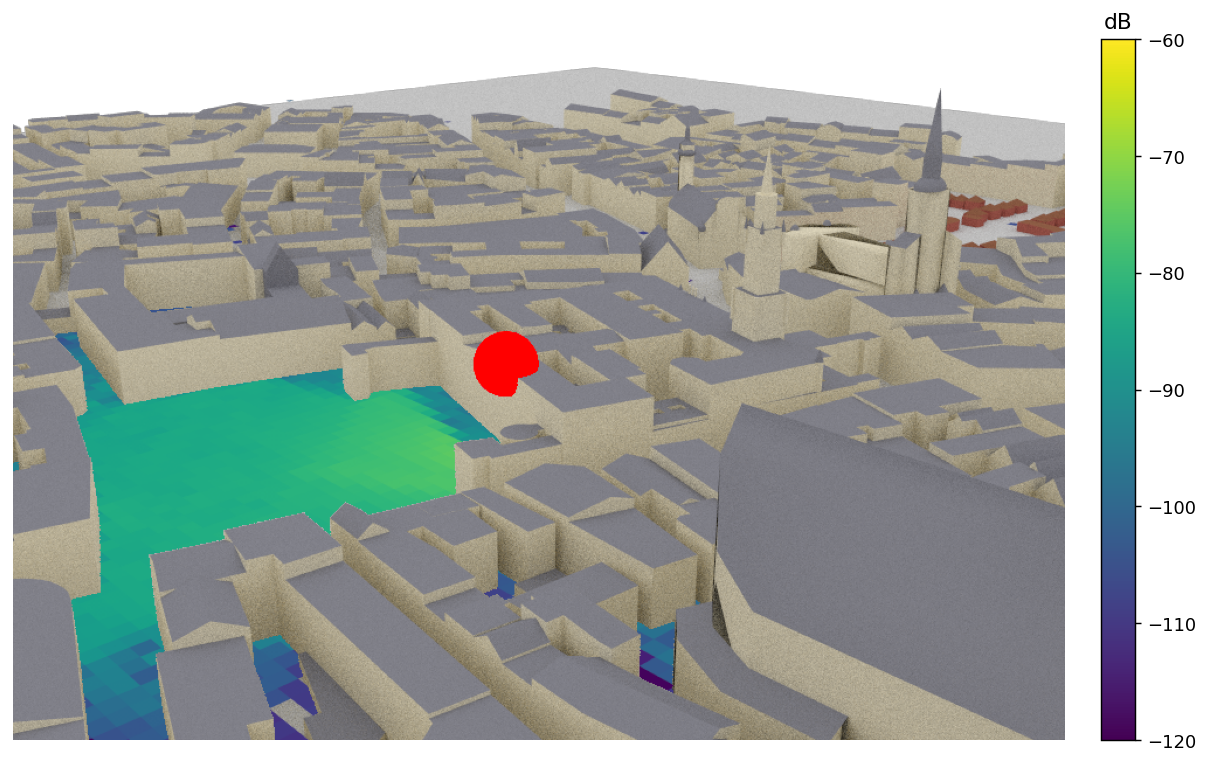
\includegraphics[width=0.5\textwidth]{img/sionna_kapsama3b.png}
\caption{Radio map computed with Sionna RT (path gain, dB). The red sphere is the transmitter (gNB); behind the buildings the signal becomes clearly weaker.}
\end{figure}

\subsection{Assessment and next steps}
Sionna 1.2.2 and Sionna RT were installed in two different environments (Ubuntu 22.04 and Windows 11), the verification scripts finished without errors and the project scripts produced the expected results. Limitations: no GPU was used (CPU only); the radar is a simplified model, not a full 3GPP channel model. Feeding Sionna RT output into ns-3 (the SioLENA module) was \textbf{not tried}. Next steps:
\begin{itemize}
\item Study the \texttt{radar()} function of the radar code (range and velocity estimation with a 2D FFT) line by line.
\item Change the residual self-interference value (\texttt{X\_SI\_DB}) and measure its effect on detection probability.
\item Compare the detection probability and error curves with the targets of TR~38.765 ($P_{md}\le 5\%$).
\end{itemize}

% ------------------------------------------------------------------ 5
\section{Overall Assessment}
All three tools were installed and their verification outputs gave the expected results. The tools complement each other: Sionna measures the \emph{gain} of sensing, while ns-3 and OCUDU measure the \emph{cost} on communication. Known limitations: 5G-LENA has no ready-made sensing model (how to represent the sensing load in ns-3 is still to be chosen); no end-to-end test (srsUE + Open5GS) was run on OCUDU; Sionna ran without a GPU and its radar model is simplified; connecting Sionna RT to ns-3 (SioLENA) was not tried.

\begingroup\sffamily\small
\begin{xltabular}{\textwidth}{@{}p{3.6cm}X@{}}
\toprule
\textbf{Team member} & \textbf{Work in the next phase} \\
\midrule
\taha & Study of 3GPP TR 38.765, metric dictionary, a common definition of $\alpha$ across the three tools, report \\
\aziz & ns-3: user-count and bandwidth sweeps, scheduler comparison, choice of how to represent the sensing load \\
\fatih & OCUDU: PRS-period and multi-user experiments; examination of the effect of PRS on PDSCH in the scheduler code \\
\nihat & Sionna: study of the radar model; comparison of detection probability and error curves with the 3GPP targets \\
\bottomrule
\end{xltabular}
\endgroup
\end{document}
